\documentclass[11pt,a4paper]{article}
\usepackage[utf8]{inputenc}
\usepackage[T1]{fontenc}
\usepackage{lmodern}
\usepackage[margin=2.5cm]{geometry}
\usepackage{amsmath,amssymb}
\usepackage{booktabs,array,tabularx}
\usepackage{graphicx}
\usepackage{enumitem}
\usepackage{microtype}
\usepackage[hidelinks]{hyperref}
\setlist{itemsep=2pt,topsep=4pt}
\renewcommand{\arraystretch}{1.12}

\newcommand{\aegis}{AEGIS-Net}

\title{\aegis: Two-Stage IoT Intrusion Detection on CICIoT2023\\[2pt]
\large Multi-Resolution Bin Embeddings for Rare Attack Classes}
\author{%
  \textbf{Tran Le Nam Kha, Duong Khac Huy, Bui Ta Thanh Quang,}\\
  \textbf{Nguyen Tuan Anh, Le Nhat Tung}\\[6pt]
  FPT University, Vietnam \quad (course DAP391m, Group 24)\\[3pt]
  {\small duongkhachuy1105@gmail.com, tranlenamkha50@gmail.com, zanhdubaii@gmail.com,}\\
  {\small buitathanhquang@gmail.com, tungln4@fpt.edu.vn}}
\date{\today}

\begin{document}
\maketitle

\begin{abstract}
\noindent\textbf{Background:} IoT networks are exposed to high-volume attacks, and an intrusion detection system (IDS) must first decide whether traffic is malicious (Stage~1) and then identify the attack family (Stage~2). Rare attack families are the hardest part of both stages: gradient-boosted trees usually isolate them well, while neural networks tend to blur them into their neighbours.

\noindent\textbf{Objective:} This study proposes \aegis, a tabular neural network designed for rare intrusion classes, and tests whether it can match or beat 14 machine-learning (ML) and deep-learning (DL) baselines under one identical protocol on CICIoT2023.

\noindent\textbf{Methods:} \aegis{} encodes every feature with a multi-resolution bin embedding (4{,}096 quantile bins, summed over a dyadic hierarchy of 13 levels), regularises fine bins towards their parents with coarse-to-fine shrinkage, and averages a 4-member BatchEnsemble. All 15 models were trained on the same 500{,}000 rows for 20 epochs (DL) or early-stopped rounds (trees), with 5 seeds, and scored on 2{,}924{,}221 held-out rows. The 34 CICIoT2023 labels were grouped into 8 families. The main metric is macro F1.

\noindent\textbf{Results:} \aegis{} ranked first on all three tasks: Stage~1 (binary) 0.9267 vs.\ 0.9256 for CatBoost, Stage~2 (attack type) 0.7446 vs.\ 0.7423 for XGBoost, and 8-class 0.7260 vs.\ 0.7228 for XGBoost, winning on 5 of 5 seeds each time. It was 0.011--0.023 ahead of the best other neural network. The margin over the best tree model is small (0.001--0.003), and after a shared decision-calibration step XGBoost matches it on the 8-class task (0.7327 vs.\ 0.7316). Ablation shows that the bin embedding ($-0.022$) and the shrinkage ($-0.014$) carry the gain, while the ensemble adds nothing measurable on this dataset.

\noindent\textbf{Conclusion:} Multi-resolution bin embeddings close most of the gap between neural networks and gradient-boosted trees on CICIoT2023, but they do not open a clear lead, and the hardest rare class (BruteForce) stays hard for every model.

\medskip
\noindent\textbf{Keywords:} IoT intrusion detection; CICIoT2023; tabular deep learning; rare attack classes; quantile bin embedding; benchmark
\end{abstract}

%=====================================================================
\section{Introduction}

\subsection{Background}
Internet of Things (IoT) deployments put large numbers of weakly protected devices on shared networks, which makes them a preferred source and target of flooding, scanning, spoofing and botnet traffic. CICIoT2023 \cite{neto2023ciciot} responds to this with a dataset of 33 attacks launched against a 105-device IoT topology, recorded as flow-level features. A practical IDS built on such data answers two questions in sequence: is this traffic an attack (Stage~1), and if so, which kind (Stage~2).

\subsection{Research problem}
Flow-level IDS data is tabular, and on tabular data gradient-boosted trees such as XGBoost \cite{chen2016xgboost}, LightGBM \cite{ke2017lightgbm} and CatBoost \cite{prokhorenkova2018catboost} remain the reference models; neural networks often trail them \cite{grinsztajn2022trees,shwartz2022tabular}. The gap is largest on rare attack families. Their signature is frequently a narrow value band of one or two features, for example a payload size that always falls inside a band about 1\% wide. A tree isolates such a band with two splits. A network that sees the raw number, or a smooth function of it, must learn a very sharp function of a continuous input and tends to blur the band into its neighbours, so the rare class is lost.

\subsection{Research gap}
Two things are missing from the current picture. First, IoT-IDS studies commonly evaluate a few models under different splits, preprocessing and tuning budgets, so a reported difference cannot be attributed to the algorithm itself \textbf{[add IDS-specific citations from your literature review]}. Second, existing numerical-feature embeddings for tabular networks, such as piece-wise linear and target-bin encodings \cite{gorishniy2022embeddings}, use one bin resolution. A fine resolution isolates narrow bands but over-fits bins that few rows touch, and a coarse resolution does the opposite. Which resolution suits rare intrusion classes has not been compared under a fair protocol on CICIoT2023.

\subsection{Research objectives}
This study therefore (i) proposes \aegis, which keeps all resolutions at once and lets the data decide how deep to go, and (ii) benchmarks it against 14 ML and DL baselines on CICIoT2023 under one protocol, so that every difference in the results can be attributed to the model.

\subsection{Research questions}
\begin{description}[leftmargin=1.2cm,style=nextline]
  \item[RQ1] Under an identical protocol, does \aegis{} outperform the ML and DL baselines on Stage~1 (benign vs.\ attack), Stage~2 (attack family) and the 8-class task?
  \item[RQ2] How does the gap between neural networks and gradient-boosted trees look on rare attack families, and does \aegis{} narrow it?
  \item[RQ3] Which components of \aegis{} (bin embedding, coarse-to-fine shrinkage, ensemble) account for its performance, and at what computational cost?
\end{description}

\subsection{Contributions}
\begin{enumerate}
  \item \aegis, a tabular network that combines a multi-resolution bin embedding, coarse-to-fine shrinkage and a BatchEnsemble.
  \item A fair benchmark of 15 models (8 ML, 7 DL including \aegis) on CICIoT2023: same split, same 500{,}000 fit rows, same class weights, fixed defaults, 5 seeds, scored on 2{,}924{,}221 test rows.
  \item An ablation and per-class analysis that states where the gain comes from and where it does not (BruteForce, the ensemble, and the calibrated decision).
\end{enumerate}

%=====================================================================
\section{Related Work}

\paragraph{Intrusion datasets.} NSL-KDD \cite{tavallaee2009nslkdd} and UNSW-NB15 \cite{moustafa2015unsw} have long served as IDS benchmarks. CICIoT2023 \cite{neto2023ciciot} is larger and IoT-specific, with 33 attacks in seven categories plus benign traffic, which makes class imbalance a central difficulty.

\paragraph{Tree ensembles.} Boosted trees \cite{chen2016xgboost,ke2017lightgbm,prokhorenkova2018catboost} handle heterogeneous, skewed features and sharp thresholds without feature engineering. Large benchmarks find that they still beat neural networks on medium-sized tabular data, largely because networks are biased towards smooth functions \cite{grinsztajn2022trees,shwartz2022tabular}.

\paragraph{Deep learning for tabular data.} Residual MLPs and the FT-Transformer \cite{gorishniy2021revisiting} set the strong neural baselines. Embedding numerical features, with periodic or quantile-bin encodings, is the most effective single change to an MLP \cite{gorishniy2022embeddings}. BatchEnsemble \cite{wen2020batchensemble} and TabM \cite{gorishniy2025tabm} add cheap implicit ensembles on top.

\paragraph{Multi-resolution encodings.} Instant-NGP \cite{muller2022instant} sums lookup tables at several resolutions to represent sharp detail in 3-D graphics. \aegis{} transfers this idea to tabular features and adds coarse-to-fine shrinkage so that sparsely populated fine bins fall back on their parent bin. To our knowledge this combination has not been published for tabular intrusion data, but this is not proof of uniqueness.

\paragraph{Gap.} Prior work either compares few models or uses a single bin resolution. This study compares 15 models under one protocol and tests a multi-resolution alternative.

%=====================================================================
\section{Methodology}

\subsection{Research framework}
Every model goes through the same pipeline, so differences in the results come from the model and not from the data handling:
\begin{enumerate}
  \item Read the CICIoT2023 CSV files, group the 34 labels into 8 families, remove duplicates and label collisions.
  \item Drop constant and highly correlated features, clip, transform and standardise the rest.
  \item Split into train, validation and test by blocks of consecutive rows (70/15/15, seed 42).
  \item Draw one class-aware sample of 500{,}000 training rows, shared by all models and seeds.
  \item Train each model with fixed default hyper-parameters, 5 seeds, and select the epoch or boosting round on the validation split.
  \item Score on the full test split, raw and after one shared calibration step.
\end{enumerate}
Three tasks are scored for every model. \textbf{Stage~1 (binary)} separates benign from attack traffic. \textbf{Stage~2 (attack type)} names the attack family on attack rows only. The \textbf{8-class task} solves both at once. Stages~1 and~2 are evaluated as separate tasks; a cascaded Stage~1~$\rightarrow$~Stage~2 pipeline was not run end to end (Section~\ref{sec:limits}).

The research questions map to the evidence as follows (Table~\ref{tab:trace}).

\begin{table}[h]
\centering\small
\caption{Research traceability matrix.}\label{tab:trace}
\begin{tabular}{@{}llllr@{}}
\toprule
RQ & Method & Experiment & Result & Discussion \\
\midrule
RQ1 & Unified benchmark & 15 models, 3 tasks, 5 seeds & Tables~\ref{tab:main}, \ref{tab:sec} & \ref{sec:findings} \\
RQ2 & Per-class F1 & 8 families, raw and calibrated & Table~\ref{tab:perclass} & \ref{sec:findings}, \ref{sec:previous} \\
RQ3 & Ablation and cost & 4 variants; fit time, latency, size & Tables~\ref{tab:ablation}, \ref{tab:cost} & \ref{sec:theory}, \ref{sec:practice} \\
\bottomrule
\end{tabular}
\end{table}

\subsection{Dataset}
CICIoT2023 \cite{neto2023ciciot} contains flow-level records of 33 attacks and benign traffic. The 34 raw labels were grouped by name prefix into 8 families: Benign, DDoS, DoS, Mirai, Recon, BruteForce, Spoofing (including man-in-the-middle) and Web-based. The task is supervised classification on numeric flow features.

\textbf{[To fill from your run log (\texttt{[data]} lines of \texttt{main.py}): rows read, rows kept after de-duplication, number of features after filtering.]}

\subsection{Data preprocessing}
\begin{enumerate}
  \item Exact duplicate rows were removed (first kept); rows with identical features but different labels were dropped.
  \item Text columns, if any, were one-hot encoded for the 12 most frequent values plus ``other''.
  \item For each pair of features with absolute correlation above 0.98, one was dropped; constant features were dropped.
  \item Values were clipped to the 0.01\% and 99.99\% quantiles; non-negative features with absolute skew above 2 received a signed log transform.
  \item Features were standardised (scaler fitted on up to 100{,}000 rows per class) and clipped at $\pm 10$ standard deviations.
  \item The split uses blocks of up to 512 consecutive rows, so neighbouring flows from the same capture stay on one side of the split. The validation split provides 200{,}000 rows to choose the best epoch or round and 500{,}000 rows to fit the decision threshold and class biases. The test split was never used for any choice.
\end{enumerate}

\subsection{\aegis}
\aegis{} has three parts.

\paragraph{Multi-resolution bin embedding (MRBE).} Each feature is cut into $2^{12}=4{,}096$ quantile bins. A value $x$ is embedded as the sum, over the dyadic hierarchy of its bin (whole range, halves, quarters, down to the finest bin), of one learned vector per level, plus a linear term:
\begin{equation}
  e(x) = W x + \sum_{l=0}^{L} T_l\!\left[\, \mathrm{bin}_L(x) \gg (L-l) \,\right], \qquad L = 12 .
\end{equation}
Coarse levels share statistical strength across many rows; fine levels can memorise a narrow band. The value is encoded exactly by a lookup, so the sharp-function problem of Section~1.2 does not arise in the embedding, and the layers above remain an ordinary smooth network. Each bin vector has 8 dimensions.

\paragraph{Coarse-to-fine shrinkage.} A penalty pulls finer levels harder towards zero, so a fine bin that few training rows touch reverts to its parent bin:
\begin{equation}
  \mathcal{R} = \lambda \sum_{l=0}^{L} g^{\,l}\, \overline{T_l^{2}}, \qquad \lambda = 0.03,\; g = 2 .
\end{equation}

\paragraph{BatchEnsemble.} On top of the embedding sit a stem layer and two residual LayerNorm--GELU blocks of width 256, shared by 4 ensemble members that differ only by rank-1 scalings and biases \cite{wen2020batchensemble}. The members' probabilities are averaged. The embedding tables use a $10\times$ larger learning rate and no weight decay, since the shrinkage penalty plays that role. The model has about 2.51 million parameters, almost all in the bin tables.

The design reuses quantile-bin embeddings \cite{gorishniy2022embeddings}, multi-resolution lookup tables \cite{muller2022instant} and BatchEnsemble \cite{wen2020batchensemble,gorishniy2025tabm}; the combination with shrinkage is the contribution.

\subsection{Compared models}
\begin{table}[h]
\centering\small
\caption{Compared models and their fixed settings.}\label{tab:models}
\begin{tabularx}{\textwidth}{@{}lXX@{}}
\toprule
Family & Models & Fixed settings \\
\midrule
ML (5) & Logistic Regression, Gaussian Naive Bayes, Decision Tree, Random Forest, Extra Trees & forests: 100 trees \\
ML, boosted (3) & XGBoost, LightGBM, CatBoost \cite{chen2016xgboost,ke2017lightgbm,prokhorenkova2018catboost} & XGBoost: eta 0.08, depth 8; LightGBM: lr 0.08, 127 leaves; CatBoost: lr 0.1, depth 8; early stopping on the validation split (patience 50, at most 2{,}000 rounds) \\
DL baselines (6) & Residual MLP, 1-D CNN, Bi-GRU, ChebyKAN, FT-Transformer \cite{gorishniy2021revisiting}, TabM \cite{gorishniy2025tabm} & one shared training loop \\
DL, proposed (1) & \aegis & levels 12, $d=8$, width 256, 2 blocks, 4 members \\
\bottomrule
\end{tabularx}
\end{table}
No model, \aegis{} included, was tuned on CICIoT2023. Tree models and baselines use fixed defaults; the three main knobs of \aegis{} (levels, shrinkage, learning-rate multiplier) were chosen earlier on UNSW-NB15 \cite{moustafa2015unsw}, and CICIoT2023 was not available during development.

\subsection{Experimental setup}
All neural models share one loop: exactly 20 epochs, AdamW \cite{loshchilov2019adamw} with learning rate $2\times10^{-3}$ and weight decay $10^{-4}$, 5\% linear warm-up then cosine decay, batch size 2{,}048, gradient clipping at 1.0, EMA weights (decay 0.999), weighted focal loss \cite{lin2017focal} ($\gamma=2$) with label smoothing 0.05. The epoch with the best macro F1 on the 200{,}000-row monitor split is kept. All models use class weights proportional to $(\text{class frequency})^{-0.5}$ and the same 499{,}996 fit rows. Every model is run with seeds 42--46; the data split and fit rows are fixed (seed 42), so the reported standard deviation reflects training randomness only. Models whose training is deterministic (Logistic Regression, Naive Bayes) show zero variance.

\subsection{Evaluation metrics}
The main metric is macro F1, the unweighted mean of per-class F1, because it counts a class of 1{,}875 test rows as much as one of 1.7 million:
\begin{equation}
  \mathrm{F1}_{\mathrm{macro}} = \frac{1}{C}\sum_{c=1}^{C} \frac{2\,P_c R_c}{P_c + R_c}.
\end{equation}
Higher is better. \textbf{F1 raw} uses the argmax decision. \textbf{F1 cal.} applies one log-bias per class fitted on the validation split, identical for every model; for Stage~1 a threshold tuned on the same split is always used. Accuracy, balanced accuracy, Matthews correlation coefficient (MCC), recall and false-positive rate (FPR) are reported as secondary metrics, together with fit time, inference time per 1{,}000 rows and parameter count.

%=====================================================================
\section{Results}
\aegis{} ranks first among 15 models on all three tasks, but its margin over the best tree model is 0.001--0.003 macro F1. All numbers below are mean $\pm$ standard deviation over seeds 42--46 on the full test split of 2{,}924{,}221 rows.

\subsection{Dataset analysis}
The test split is dominated by flooding attacks, while the two rarest families together make up under 0.2\% of the rows (Table~\ref{tab:classes}). Benign traffic is only 5.4\% of the test rows, which matters for the false-positive rate of Stage~1 (Section~\ref{sec:main}).

\begin{table}[h]
\centering\small
\caption{Class distribution of the test split.}\label{tab:classes}
\begin{tabular}{@{}lcc@{}}
\toprule
Class & Test rows & Share (\%) \\
\midrule
DDoS & 1{,}716{,}959 & 58.71 \\
DoS & 528{,}626 & 18.08 \\
Mirai & 353{,}162 & 12.08 \\
Benign & 156{,}929 & 5.37 \\
Recon & 97{,}971 & 3.35 \\
Spoofing & 65{,}161 & 2.23 \\
Web-based & 3{,}538 & 0.12 \\
BruteForce & 1{,}875 & 0.06 \\
\bottomrule
\end{tabular}
\end{table}

\subsection{Model performance (RQ1)}\label{sec:main}
\aegis{} has the highest macro F1 on Stage~1, Stage~2 and the 8-class task, and the best mean rank (1.00) of the 15 models. XGBoost and CatBoost tie for second (2.67). The best neural baseline, the residual MLP, is 0.011 to 0.023 behind \aegis.

\begin{table}[h]
\centering\small
\caption{Macro F1 (raw decision) of all 15 models, sorted by mean rank. Logistic Regression and Naive Bayes are deterministic and have no seed variance.}\label{tab:main}
\begin{tabular}{@{}llcccc@{}}
\toprule
Model & Type & Stage 1 (binary) & Stage 2 (attack type) & 8-class & Mean rank \\
\midrule
\textbf{\aegis}      & DL & $0.9267\pm0.0002$ & $0.7446\pm0.0004$ & $0.7260\pm0.0004$ & 1.00 \\
XGBoost              & ML & $0.9251\pm0.0002$ & $0.7423\pm0.0009$ & $0.7228\pm0.0007$ & 2.67 \\
CatBoost             & ML & $0.9256\pm0.0002$ & $0.7388\pm0.0003$ & $0.7203\pm0.0004$ & 2.67 \\
LightGBM             & ML & $0.9251\pm0.0001$ & $0.7387\pm0.0006$ & $0.7195\pm0.0006$ & 3.67 \\
Random Forest        & ML & $0.9214\pm0.0001$ & $0.7366\pm0.0006$ & $0.7171\pm0.0004$ & 5.00 \\
MLP-Res              & DL & $0.9159\pm0.0001$ & $0.7228\pm0.0006$ & $0.7034\pm0.0006$ & 6.33 \\
CNN1D                & DL & $0.9141\pm0.0002$ & $0.7157\pm0.0009$ & $0.6952\pm0.0005$ & 7.67 \\
Extra Trees          & ML & $0.9120\pm0.0001$ & $0.7216\pm0.0007$ & $0.7054\pm0.0004$ & 8.00 \\
TabM                 & DL & $0.9134\pm0.0001$ & $0.7099\pm0.0005$ & $0.6908\pm0.0002$ & 9.00 \\
ChebyKAN             & DL & $0.9128\pm0.0001$ & $0.7099\pm0.0027$ & $0.6919\pm0.0020$ & 9.33 \\
FT-Transformer       & DL & $0.9121\pm0.0002$ & $0.7043\pm0.0010$ & $0.6896\pm0.0018$ & 10.67 \\
Decision Tree        & ML & $0.8976\pm0.0001$ & $0.6735\pm0.0001$ & $0.6575\pm0.0001$ & 12.33 \\
Bi-GRU               & DL & $0.9011\pm0.0008$ & $0.6549\pm0.0090$ & $0.6391\pm0.0101$ & 12.67 \\
Logistic Regression  & ML & $0.8681$ & $0.6374$ & $0.6042$ & 14.00 \\
Naive Bayes          & ML & $0.8393$ & $0.4662$ & $0.3734$ & 15.00 \\
\bottomrule
\end{tabular}
\end{table}

The secondary metrics tell a more mixed story (Table~\ref{tab:sec}). On the 8-class task \aegis{} has the best balanced accuracy (0.7436), but XGBoost is ahead on calibrated F1 (0.7327 vs.\ 0.7316), and MCC is a tie at 0.760. On Stage~1, \aegis{} has the highest recall (0.9902) and also a higher false-positive rate (0.1131) than XGBoost (0.1012) and CatBoost (0.1021).

\begin{table}[h]
\centering\small
\caption{Finalists: secondary metrics on the 8-class task and the Stage~1 operating point.}\label{tab:sec}
\begin{tabular}{@{}lcccccc@{}}
\toprule
Model & F1 cal.\ (8-class) & Accuracy & Balanced acc. & MCC & S1 recall & S1 FPR \\
\midrule
\textbf{\aegis} & $0.7316\pm0.0067$ & 0.8510 & 0.7436 & 0.7603 & 0.9902 & 0.1131 \\
XGBoost         & $0.7327\pm0.0018$ & 0.8488 & 0.7379 & 0.7603 & 0.9889 & 0.1012 \\
CatBoost        & $0.7248\pm0.0025$ & 0.8498 & 0.7272 & 0.7605 & 0.9891 & 0.1021 \\
MLP-Res         & $0.7080\pm0.0024$ & 0.8400 & 0.7129 & 0.7446 & 0.9878 & 0.1173 \\
CNN1D           & $0.6969\pm0.0015$ & 0.8381 & 0.6995 & 0.7432 & 0.9874 & 0.1186 \\
\bottomrule
\end{tabular}
\end{table}

The finalists are the two strongest ML and the two strongest DL baselines (by mean rank, \aegis{} excluded) plus \aegis. \textbf{Answer to RQ1:} yes on raw macro F1, by a small margin over trees and a clear margin over other networks; no clear win once decisions are calibrated.

\subsection{Comparative analysis: rare classes (RQ2)}
Figure~\ref{fig:perclass} and Table~\ref{tab:perclass} show the F1 of each family. The largest per-class gain of \aegis{} is on Web-based (0.348 vs.\ 0.320 for XGBoost, $+0.028$), the second-rarest class. It also leads or ties on Spoofing, Recon, Benign, Mirai and DDoS by 0.000--0.003. It does not help on BruteForce (0.369 vs.\ 0.379 for CatBoost) or DoS (0.672 vs.\ 0.678 for XGBoost). The neural baselines lose most on the rare classes: Web-based drops to 0.268 for MLP-Res and 0.241 for CNN1D.

\begin{table}[h]
\centering\small
\caption{F1 per class, raw decision (rarest class first). Best value per row in bold.}\label{tab:perclass}
\begin{tabular}{@{}lcccccc@{}}
\toprule
Class & Test rows & XGBoost & CatBoost & MLP-Res & CNN1D & \aegis \\
\midrule
BruteForce & 1{,}875 & 0.375 & \textbf{0.379} & 0.378 & 0.355 & 0.369 \\
Web-based  & 3{,}538 & 0.320 & 0.307 & 0.268 & 0.241 & \textbf{0.348} \\
Spoofing   & 65{,}161 & \textbf{0.897} & 0.894 & 0.849 & 0.846 & \textbf{0.897} \\
Recon      & 97{,}971 & 0.778 & 0.772 & 0.763 & 0.757 & \textbf{0.780} \\
Benign     & 156{,}929 & 0.856 & 0.852 & 0.837 & 0.831 & \textbf{0.859} \\
Mirai      & 353{,}162 & \textbf{0.997} & \textbf{0.997} & \textbf{0.997} & \textbf{0.997} & \textbf{0.997} \\
DoS        & 528{,}626 & \textbf{0.678} & 0.677 & 0.658 & 0.660 & 0.672 \\
DDoS       & 1{,}716{,}959 & 0.883 & 0.884 & 0.878 & 0.876 & \textbf{0.886} \\
\bottomrule
\end{tabular}
\end{table}

\begin{figure}[h]
\centering
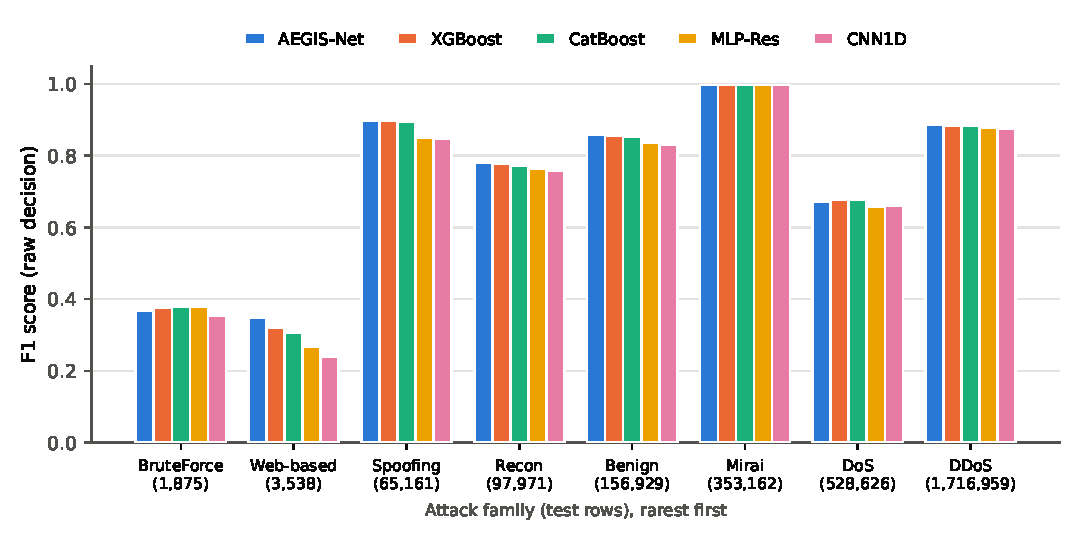
\includegraphics[width=\textwidth]{fig_perclass.pdf}
\caption{Per-class F1 (raw decision, mean of 5 seeds) on the 8-class task, classes from rarest (left) to most frequent (right), test rows in brackets. \aegis{} leads clearly only on Web-based (0.348 vs.\ 0.320 for XGBoost); on BruteForce every model stays below 0.38. Values: Table~\ref{tab:perclass}.}\label{fig:perclass}
\end{figure}

After the shared calibration the picture shifts towards trees: XGBoost reaches 0.436 on BruteForce (\aegis{} 0.398) and 0.894 on DDoS (0.886), while \aegis{} keeps the lead on Web-based (0.360 vs.\ 0.332). \textbf{Answer to RQ2:} the neural-to-tree gap on rare classes is largely closed for Web-based, where \aegis{} is 0.08--0.11 above the two neural finalists and ahead of the trees, and not closed for BruteForce, where every finalist stays below 0.44.

\subsection{Ablation and cost (RQ3)}
Removing the bins costs 0.022 macro F1 and removing the shrinkage costs 0.014. Using one ensemble member instead of four changes nothing measurable ($+0.001$). The F1 of the three rarest classes (BruteForce, Web-based, Spoofing) falls by 0.035 without bins and 0.018 without shrinkage. The ablation used a reduced protocol (60{,}000 fit rows, batch size 512, 3 seeds), so its absolute values are not comparable with Table~\ref{tab:main}.

\begin{table}[h]
\centering\small
\caption{Ablation of \aegis{} on the 8-class task (reduced protocol).}\label{tab:ablation}
\begin{tabular}{@{}lcccc@{}}
\toprule
Variant & F1 macro (raw) & Change vs.\ full & F1 macro (cal.) & Mean F1, 3 rarest \\
\midrule
Full model             & $0.7050\pm0.0013$ & --- & 0.7097 & 0.5034 \\
No shrinkage           & $0.6911\pm0.0007$ & $-0.0139$ & 0.6949 & 0.4851 \\
No bins (levels $=0$)  & $0.6832\pm0.0006$ & $-0.0218$ & 0.6844 & 0.4683 \\
1 member (no ensemble) & $0.7059\pm0.0013$ & $+0.0009$ & 0.7114 & 0.5069 \\
\bottomrule
\end{tabular}
\end{table}

The price is training time and size. \aegis{} fits in 73~s on the 8-class task, versus 27~s for XGBoost and 25--31~s for the residual MLP and the CNN, and has 2.5 million parameters. Its inference time of 0.47~ms per 1{,}000 rows is half that of XGBoost and one third of CatBoost (Table~\ref{tab:cost}).

\begin{table}[h]
\centering\small
\caption{Computational cost on the 8-class task.}\label{tab:cost}
\begin{tabular}{@{}lccc@{}}
\toprule
Model & Fit time (s) & Inference (ms / 1{,}000 rows) & Parameters \\
\midrule
\textbf{\aegis} & 73.3 & 0.47 & 2{,}510{,}496 \\
XGBoost  & 26.5 & 1.03 & 1{,}307{,}534 \\
CatBoost & 611.6 & 1.38 & 96{,}000 \\
MLP-Res  & 24.7 & 0.16 & 210{,}696 \\
CNN1D    & 30.7 & 0.66 & 59{,}179 \\
\bottomrule
\end{tabular}
\end{table}

\textbf{Answer to RQ3:} the bin embedding and the shrinkage account for the gain; the ensemble does not on CICIoT2023.

\subsection{Statistical analysis}
The five seeds change training only; the data split and fit rows are fixed. On raw macro F1, \aegis{} beats the strongest competitor on all 5 paired seeds on every task: $+0.0011\pm0.0003$ over CatBoost on Stage~1, $+0.0023\pm0.0011$ over XGBoost on Stage~2, and $+0.0032\pm0.0007$ over XGBoost on the 8-class task (paired differences, mean $\pm$ standard deviation). After calibration the 8-class difference to XGBoost is $-0.0012\pm0.0080$ with 2 wins in 5, and the Stage~2 difference is $+0.0026\pm0.0035$ with 3 wins in 5. No significance test was run; with 5 seeds and one split, the raw-F1 margins are consistent but small, and the calibrated margins are within noise.

%=====================================================================
\section{Discussion}

\subsection{Main findings}\label{sec:findings}
\paragraph{Finding.} \aegis{} is first on all three tasks in raw macro F1, ahead of the best tree by 0.001--0.003 and of the best other network by 0.011--0.023, and it wins on every paired seed.

\paragraph{Interpretation.} The result suggests that the neural-network penalty on this dataset is largely a resolution problem. A network that encodes values exactly through bins reaches tree-level accuracy without trees' thresholds. It does not say neural networks are now better: after calibration the 8-class advantage over XGBoost disappears ($-0.0012\pm0.0080$).

\paragraph{Explanation.} The ablation supports a resolution mechanism. Removing the bins costs 0.022 overall and 0.035 on the three rarest classes, and the clearest per-class gain is on Web-based ($+0.028$ over XGBoost), a class of 3{,}538 test rows. We read this as the bin lookup letting the network isolate narrow value bands that smooth encodings blur, as intended in Section~1.2; we did not inspect which features carry those bands, so this remains a hypothesis. Shrinkage adds 0.014, consistent with its role of stopping sparse fine bins from over-fitting.

\paragraph{Where it does not help.} BruteForce stays near 0.37--0.44 F1 for every finalist, and DoS is slightly better with trees (0.678 vs.\ 0.672). When all models fail alike on one class, the limit is more likely in the features or the labels (for example overlap with other families) than in model capacity. This was not tested here.

\subsection{Comparison with previous studies}\label{sec:previous}
Our earlier runs of the same code base under a reduced protocol (60{,}000 fit rows, 3 seeds) show the same pattern as the literature \cite{grinsztajn2022trees,shwartz2022tabular}: on UNSW-NB15 \cite{moustafa2015unsw} \aegis{} ranked first on all three tasks, while on NSL-KDD \cite{tavallaee2009nslkdd} gradient-boosted trees stayed ahead of it by 0.0005--0.02. CICIoT2023 sits between the two. \aegis{} leads, but only narrowly over trees, and CICIoT2023 played no role in choosing its hyper-parameters, which makes it a fairer check than UNSW-NB15. The finding that quantile-bin embeddings are the most effective single change for tabular networks \cite{gorishniy2022embeddings} is consistent with the ablation, where removing bins is the most damaging step. Unlike on UNSW-NB15, where a single member lost 0.014, the 4-member ensemble gave no gain here ($+0.001$ for one member), so TabM-style ensembling \cite{gorishniy2025tabm} is not what lifts \aegis{} on this dataset.

\subsection{Theoretical implications}\label{sec:theory}
The results suggest that, for flow-level intrusion data, the gap between boosted trees and networks can be narrowed by changing the input representation rather than the architecture: the networks above the embedding are standard residual blocks. They also suggest that keeping every resolution and shrinking the fine ones is a workable alternative to choosing one bin count per feature, since a single fine resolution would over-fit bins with few rows.

\subsection{Practical implications}\label{sec:practice}
For a deployed IoT IDS, accuracy is not the only constraint. \aegis{} scores 0.47~ms per 1{,}000 rows, faster than XGBoost (1.03~ms) and CatBoost (1.38~ms), and its 2.5 million parameters occupy roughly 10~MB at 32-bit precision, so inference cost is not a barrier. Training is slower than XGBoost (73~s vs.\ 27~s here). Stage~1 needs a closer look: all models reach recall near 0.99 but with a false-positive rate around 0.10--0.12, because the decision threshold was tuned for F1 and benign traffic is only 5.4\% of the rows. An operator who cares about false alarms should choose the threshold on a target FPR; the FPR of \aegis{} (0.1131) is slightly above the trees' (0.101--0.102) at the F1-optimal point. Since the margin over trees is small, gradient-boosted trees remain a strong, cheaper default when training time matters.

\subsection{Limitations}\label{sec:limits}
\begin{itemize}
  \item \textbf{One dataset and one split.} Seeds vary training only. Block splitting keeps neighbouring flows together but cannot rule out dependence between train and test flows from the same capture.
  \item \textbf{Small margins, no formal test.} Raw-F1 margins are consistent over 5 seeds but 0.001--0.003; calibrated margins are within noise.
  \item \textbf{Fixed defaults for all models.} No baseline was tuned, and the \aegis{} knobs came from UNSW-NB15. Tuned trees could widen or close the gap.
  \item \textbf{Stages evaluated separately.} Stage~2 is trained and scored on attack rows only. A cascade in which Stage~1 errors reach Stage~2 was not run, so its end-to-end performance is unknown.
  \item \textbf{Reduced-protocol ablation.} It used 60{,}000 fit rows and 3 seeds, and the ensemble conclusion may change at full scale.
  \item \textbf{Timing from one machine.} Fit and inference times are indicative; confirm the hardware (the Colab notebook shows an NVIDIA A100 40~GB) before quoting them.
\end{itemize}

%=====================================================================
\section{Conclusion}

\subsection{Summary}
This study compared \aegis{} with 14 ML and DL models on CICIoT2023 under one protocol. \aegis{} ranked first on Stage~1 (0.9267), Stage~2 (0.7446) and the 8-class task (0.7260) in raw macro F1, closing most of the gap between networks and boosted trees. The gain comes from the multi-resolution bin embedding and the shrinkage, not from the ensemble. The advantage over trees is small and vanishes after calibration, and BruteForce remains hard for every model.

\subsection{Contributions}
We contribute the \aegis{} design, a fair 15-model benchmark on CICIoT2023 with 5 seeds, and an ablation and per-class analysis that separates what the model improves (Web-based, overall balance) from what it does not (BruteForce, the calibrated decision).

\subsection{Future work}
Future work should (i) run the Stage~1~$\rightarrow$~Stage~2 cascade end to end, (ii) evaluate on further datasets and with several data splits, (iii) tune the baselines with the same budget, (iv) test whether the ensemble helps at full scale, and (v) inspect which features carry the narrow bands that the bins isolate, and why BruteForce resists every model.

%=====================================================================
\begin{thebibliography}{99}\small

\bibitem{neto2023ciciot} E.~C.~P. Neto, S.~Dadkhah, R.~Ferreira, A.~Zohourian, R.~Lu, A.~A. Ghorbani. CICIoT2023: A real-time dataset and benchmark for large-scale attacks in IoT environment. \emph{Sensors}, 23(13):5941, 2023.

\bibitem{tavallaee2009nslkdd} M.~Tavallaee, E.~Bagheri, W.~Lu, A.~A. Ghorbani. A detailed analysis of the KDD CUP 99 data set. \emph{IEEE Symposium on Computational Intelligence for Security and Defense Applications (CISDA)}, 2009.

\bibitem{moustafa2015unsw} N.~Moustafa, J.~Slay. UNSW-NB15: a comprehensive data set for network intrusion detection systems. \emph{Military Communications and Information Systems Conference (MilCIS)}, 2015.

\bibitem{chen2016xgboost} T.~Chen, C.~Guestrin. XGBoost: A scalable tree boosting system. \emph{KDD}, 2016.

\bibitem{ke2017lightgbm} G.~Ke et al. LightGBM: A highly efficient gradient boosting decision tree. \emph{NeurIPS}, 2017.

\bibitem{prokhorenkova2018catboost} L.~Prokhorenkova, G.~Gusev, A.~Vorobev, A.~V. Dorogush, A.~Gulin. CatBoost: unbiased boosting with categorical features. \emph{NeurIPS}, 2018.

\bibitem{grinsztajn2022trees} L.~Grinsztajn, E.~Oyallon, G.~Varoquaux. Why do tree-based models still outperform deep learning on typical tabular data? \emph{NeurIPS Datasets and Benchmarks}, 2022.

\bibitem{shwartz2022tabular} R.~Shwartz-Ziv, A.~Armon. Tabular data: Deep learning is not all you need. \emph{Information Fusion}, 81:84--90, 2022.

\bibitem{gorishniy2021revisiting} Y.~Gorishniy, I.~Rubachev, V.~Khrulkov, A.~Babenko. Revisiting deep learning models for tabular data. \emph{NeurIPS}, 2021.

\bibitem{gorishniy2022embeddings} Y.~Gorishniy, I.~Rubachev, A.~Babenko. On embeddings for numerical features in tabular deep learning. \emph{NeurIPS}, 2022.

\bibitem{wen2020batchensemble} Y.~Wen, D.~Tran, J.~Ba. BatchEnsemble: An alternative approach to efficient ensemble and lifelong learning. \emph{ICLR}, 2020.

\bibitem{gorishniy2025tabm} Y.~Gorishniy, A.~Kotelnikov, A.~Babenko. TabM: Advancing tabular deep learning with parameter-efficient ensembling. \emph{ICLR}, 2025.

\bibitem{muller2022instant} T.~M\"uller, A.~Evans, C.~Schied, A.~Keller. Instant neural graphics primitives with a multiresolution hash encoding. \emph{ACM Transactions on Graphics}, 41(4), 2022.

\bibitem{lin2017focal} T.-Y. Lin, P.~Goyal, R.~Girshick, K.~He, P.~Doll\'ar. Focal loss for dense object detection. \emph{ICCV}, 2017.

\bibitem{loshchilov2019adamw} I.~Loshchilov, F.~Hutter. Decoupled weight decay regularization. \emph{ICLR}, 2019.

\end{thebibliography}

\end{document}
